\documentclass{beamer}

\usefonttheme{professionalfonts}
% \usepackage{unicode-math}

%\usepackage{latexsym}
%\usepackage{amsmath}
%\usepackage{amsfonts}
\usepackage{verbatim}
\usepackage{graphicx}
\usepackage{iwona}

%%% xetex

\usepackage{fontspec}
\setmainfont[Ligatures=TeX]{Linux Libertine O}
\newfontfamily\fallbackfont{Asana Math}
%\setmonofont{Asana Math}
\setmonofont{DejaVu Sans Mono}
\usepackage{newunicodechar}


%\usetheme{Amsterdam}
%\usetheme{Madrid} 
\usetheme{progressbar}
%\usetheme{default}
%\usetheme{Warsaw}
%\usetheme{Bergen} % This template has nagivation on the left
%\usetheme{Frankfurt} % Similar to the default 
%with an extra region at the top.
%\usecolortheme{seahorse} % Simple and clean template
%\usetheme{Darmstadt} % not so good
% Uncomment the following line if you want %
% page numbers and using Warsaw theme%
% \setbeamertemplate{footline}[page number]
%\setbeamercovered{transparent}
\setbeamercovered{invisible}
% To remove the navigation symbols from 
% the bottom of slides%
\setbeamertemplate{navigation symbols}{} 
%

\progressbaroptions{imagename=logic.png}

%\usepackage{bm}         % For typesetting bold math (not \mathbold)
%\logo{\includegraphics[height=0.6cm]{yourlogo.eps}}
%

\title[Real Encodings]{Real Encodings of Boolean Formulas and their Algebraic Representation}
\author{\textsc{M. Barney}}
\institute[U of New Mexico]
{
University of New Mexico \\
\medskip
{\emph{mbunm12@cs.unm.edu}}
}
\date{\today}


%%%%%%%%%%%%%%%%%%%%%%%%%%%%

\begin{document}

%%%%%%%%%%%%%%%%%%%
\begin{frame}
\titlepage
\end{frame}
%%%%%%%%%%%%%%%%%%%

%%%%%%%%%%%%%%%%%%%
\begin{frame}
\frametitle{Introduction}
\begin{block}
{Boolean Logic} 

Boolean logic is the logic of ``true'' and ``false''.

\begin{center}
\begin{tabular}{|c|c|c|}\hline
\(A\) & \( \land\) & \( B\) \\ \hline
  1   &      1     &    1   \\ \hline
  0   &      0     &    1   \\ \hline
  1   &      0     &    0   \\ \hline
  0   &      0     &    0   \\ \hline
\end{tabular}
\end{center}

%\begin{center}
%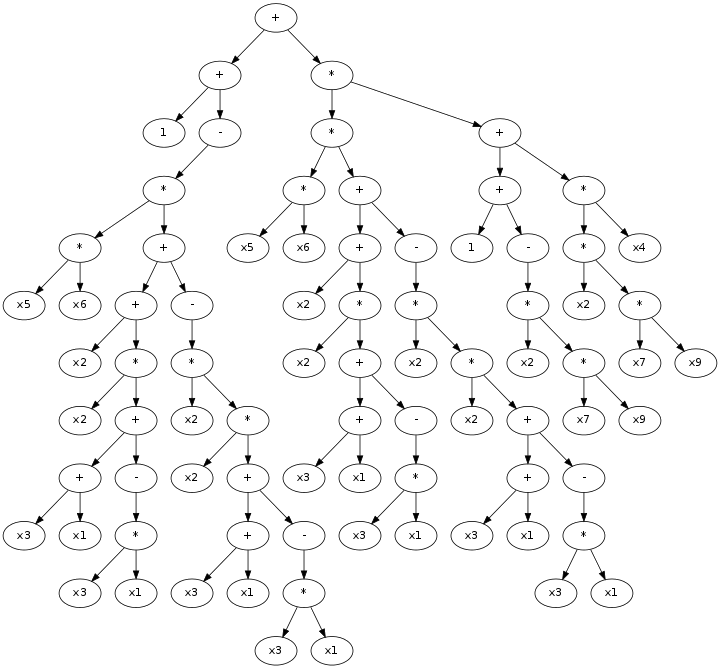
\includegraphics[width=0.25\textwidth]{imp.png}
%\end{center}

\end{block}
\end{frame}
%%%%%%%%%%%%%%%%%%%

%%%%%%%%%%%%%%%%%%%
\begin{frame}
\frametitle{Applications}
\begin{block}
{SAT} 

Determine if some arbitrary boolean formula, \(\mathcal{F}\), is satisfiable or not.

\end{block}


\begin{alertblock}
{Satisfiability}
A formula \(\mathcal{F}\) is satisfiable \textbf{iff} there exists some assignment of truth values, \(\mathcal{M}\), such that \(\mathcal{F}_{\mathcal{M}} \models \top\)
\end{alertblock}

\end{frame}
%%%%%%%%%%%%%%%%%%%

%%%%%%%%%%%%%%%%%%%
\begin{frame}
\frametitle{Example}
\begin{exampleblock}
{SAT, UNSAT} 

\begin{itemize}
\item \((A \Rightarrow B)\) --- SAT
\item \((((A \Rightarrow B) \land A) \Rightarrow B)\) --- SAT
\item \((A \land \neg A)\) --- UNSAT
\end{itemize}
\end{exampleblock}

\begin{alertblock}
{Contradictions}

A contradiction, \(\bot\), is any formula for which \emph{no} assignment of true and false can make the formula true.

All contradictions are UNSAT.  

Hence a formula \(\mathcal{F}\) is SAT \textbf{iff} \(\mathcal{F} \not \equiv \bot\) 
\end{alertblock}

\end{frame}
%%%%%%%%%%%%%%%%%%%

%%%%%%%%%%%%%%%%%%%
\begin{frame}
\frametitle{Modern SAT Solvers}
\begin{block}
{DPLL} 

Modern SAT solvers implement variations of the ``David-Putnam-Logemann-Loveland'' algorithm for determining satisfiability of a boolean expression.

Modern implementations are very sophisticated, employing back-tracking, and other heuristics to speed up solver run times.

\end{block}
\end{frame}
%%%%%%%%%%%%%%%%%%%

%%%%%%%%%%%%%%%%%%%
\begin{frame}
\frametitle{DPLL}
\begin{alertblock}
{Complete} 

DPLL is \textbf{complete} --- that is, for any arbitrary boolean expression, it is guaranteed to terminate with a solution, SAT, or UNSAT.

\end{alertblock}
\end{frame}
%%%%%%%%%%%%%%%%%%%

%%%%%%%%%%%%%%%%%%%
\begin{frame}
\frametitle{Complexity}
\begin{block}
{Unfortunately \ldots} 

Since SAT solving arbitrary boolean expressions will contain instances of 3-SAT problems, general SAT solving is NP-complete.

In the worst case, DPLL, and other complete algorithms run in exponential time, as the method eventually devolves to truth-table enumeration (``bit-blasting'').

For \emph n boolean variables, the size of a truth table is \(2^n\).

\end{block}
\end{frame}
%%%%%%%%%%%%%%%%%%%

%%%%%%%%%%%%%%%%%%%
\begin{frame}{fragile}
\frametitle{My Method}
\begin{block}
{Real Encodings}

\begin{enumerate}
\item {\tiny Consider a boolean expression's truth table as an infinitely long, \emph{repeating} bit vector, e.g.: \(A \land B = \overline{1000}\) }
\item {\tiny Define a coding for the \emph{i}th bit in a bit vector, \emph{b}: \( f(b_i) = \begin{cases} \frac{1}{2^{2i-1}} & \text{ if } b_i = 1\\ 0  & \text{ otherwise } \end{cases}\) where \emph{i} \(\geq\) 1 }
\item {\tiny Define a geometric sum for a bit vector, \emph b: }
  \[
  \sum_{i=1}^\infty b_i \frac{1}{2^{2i-1}}
  \]
\item {\tiny Then the real encoding for a boolean formula, \(\mathcal{F}\), with bit vector \(b\), is given by the following:}
  \[
  \mathcal{E}(\mathcal{F} = b) = \sum_{i=1}^\infty
 f(b_i) = \sum_{i=1}^\infty \frac{b_i}{2^{2i-1}}
  \]
\end{enumerate}


\end{block}
\end{frame}
%%%%%%%%%%%%%%%%%%%

\begin{comment}
\begin{cases} 
\frac{1}{2^{2i-1}} & \text{ if } b_i = 1\\ 0  & \text{ otherwise }
 \end{cases}
\end{comment}

%%%%%%%%%%%%%%%%%%%
\begin{frame}
\frametitle{Example Encodings}
\begin{exampleblock}
{Some Example Encodings}

\begin{itemize}
\item \(  \mathcal{E}(A  = \overline{10}) = \frac{2}{3} \)
\item \(  \mathcal{E}(B  = \overline{1100}) = \frac{4}{5} \)
\item \(  \mathcal{E}(A \land B  = \overline{1000} ) = \frac{8}{15}\)
\item \(  \mathcal{E}(A \lor B  = \overline{1110} ) = \frac{14}{15}\)
\item \(  \mathcal{E}(A \land \neg A  = \overline{0} ) = 0\)
\item \(  \mathcal{E}(A \lor \neg A  = \overline{1} ) = 1\)
\end{itemize}

\end{exampleblock}
\end{frame}
%%%%%%%%%%%%%%%%%%%

%%%%%%%%%%%%%%%%%%%
\begin{frame}
\frametitle{Literal Encodings}
\begin{block}
{Sufficient to Encode Boolean Literals}

We shall see that once we introduce an algebraic interpretation for boolean operators, it is sufficient to just encode boolean literals, i.e., \(A, B, C, D, \ldots\), and \emph{compute} the remaining fractional encodings for non-literal formulae (if we so desire).

An important formula for obtaining the \emph{n}th boolean literal's encoding is given by:
\[
f(n) = \frac{2^{2^n}}{2^{2^n} + 1}
\]

where we index literals from 0, i.e.: \(n \geq 0\).

\end{block}
\end{frame}
%%%%%%%%%%%%%%%%%%%

%%%%%%%%%%%%%%%%%%%
\begin{frame}
\frametitle{Algebraization}
\begin{alertblock}
{Algebraic Forms of the Boolean Operators}

{\small
We actually only need to define the algebraic equivalent for a single operator, the Sheffer stroke, or NAND, as it's called by computer scientists.

Neverthless, it is useful to see the resulting algebraic expressions for the various operators:}

\begin{center}
\begin{tabular}{ll}\hline
Logical Form            & Algebraic Form\\
\(\neg A\)              & \(1 - a\)\\
\(A \land B\)           & \(ab\)\\
\(A \lor B\)            & \(a + b - ab\)\\
\(A \Rightarrow B\)     & \(1 - a + ab\)\\
\(A \Leftrightarrow B\) & \(1 - a - b + 2ab\)\\\hline
\end{tabular}
\end{center}

where \(a,b,c,\ldots\) are unique variables.

\end{alertblock}
\end{frame}
%%%%%%%%%%%%%%%%%%%

%%%%%%%%%%%%%%%%%%%
\begin{frame}
\frametitle{Sample Encoding Derivation}
\begin{exampleblock}
{Sample Derivation}

As stated earlier, we can obtain the encoding for any arbitrary boolean formula by simply substituting the appropriate literal encoding in an algebraic expression.

Given the logical formula \(A \lor B\):

\begin{enumerate}
\item \(a + b - ab \)
\item \(\frac{2}{3} + \frac{4}{5} - \frac{2}{3} \frac{4}{5} \)
\item \(\frac{22}{15} - \frac{8}{15} \)
\item \(\frac{14}{15} \)
\end{enumerate}

\end{exampleblock}
\end{frame}
%%%%%%%%%%%%%%%%%%%

%%%%%%%%%%%%%%%%%%%
\begin{frame}
\frametitle{}
\begin{block}
{}

\end{block}
\end{frame}
%%%%%%%%%%%%%%%%%%%

%%%%%%%%%%%%%%%%%%%
\begin{frame}
\frametitle{}
\begin{block}
{}

\end{block}
\end{frame}
%%%%%%%%%%%%%%%%%%%

%%%%%%%%%%%%%%%%%%%
\begin{frame}
\frametitle{}
\begin{block}
{}

\end{block}
\end{frame}
%%%%%%%%%%%%%%%%%%%

%%%%%%%%%%%%%%%%%%%
\begin{frame}
\frametitle{}
\begin{block}
{}

\end{block}
\end{frame}
%%%%%%%%%%%%%%%%%%%

%%%%%%%%%%%%%%%%%%%
\begin{frame}
\frametitle{}
\begin{block}
{}

\end{block}
\end{frame}
%%%%%%%%%%%%%%%%%%%

%%%%%%%%%%%%%%%%%%%
\begin{frame}
\frametitle{}
\begin{block}
{}

\end{block}
\end{frame}
%%%%%%%%%%%%%%%%%%%

%%%%%%%%%%%%%%%%%%%
\begin{frame}[fragile]
\frametitle{Algos}
\begin{block}
{Concrete OCaml implementation}

%\includegraphics[width=0.25\textwidth]{tableaux.png}

\begin{center}
\begin{verbatim}
<αλγος> ((a \/ ~b) & ~a) -> ~b
Parsed: (((a ∨ (¬b)) ∧ (¬a)) ⇒ (¬b))
Variables(2): a b
Algebraic form: (1 + ((−((a + ((1 + (−b)) +
 (−(a × (1 + (−b)))))) × (1 + (−a)))) +
 (((a + ((1 + (−b)) + (−(a × (1 + (−b)))))) ×
 (1 + (−a))) × (1 + (−b)))))
Algos reduced form: (1)
\end{verbatim}
\end{center}


\end{block}
\end{frame}
%%%%%%%%%%%%%%%%%%%


%%%%%%%%%%%%%%%%%%%

%%%%%%%%%%%%%%%%%%%
\begin{frame}
\frametitle{Mais}
\begin{block}
{je refuse!} 


\begin{quote}
``a writer should not allow himself to be turned into an institution'' --- \textsc{JP}
\end{quote}


\end{block}
\end{frame}
%%%%%%%%%%%%%%%%%%%

% End of slides
%\begin{frame}
%\frametitle{Bibliography}
%\bibliographystyle{plain}
%\bibliography{cs}
%\end{frame}


\end{document}
